\documentclass[]{article}
\usepackage{graphicx}
\usepackage{amsmath}

%opening

\begin{document}

\section{FSA and Regular Expressions}
\subsection{Finite State Automata}
\begin{itemize}
	\item A finite state automaton (FSA) is a directed graph with a finite number of nodes.

	\item A FSA is described by a 5 tuple: (states, alphabet, initial state, final state, transition)
	
	\begin{figure}[h!]
		\begin{center}
			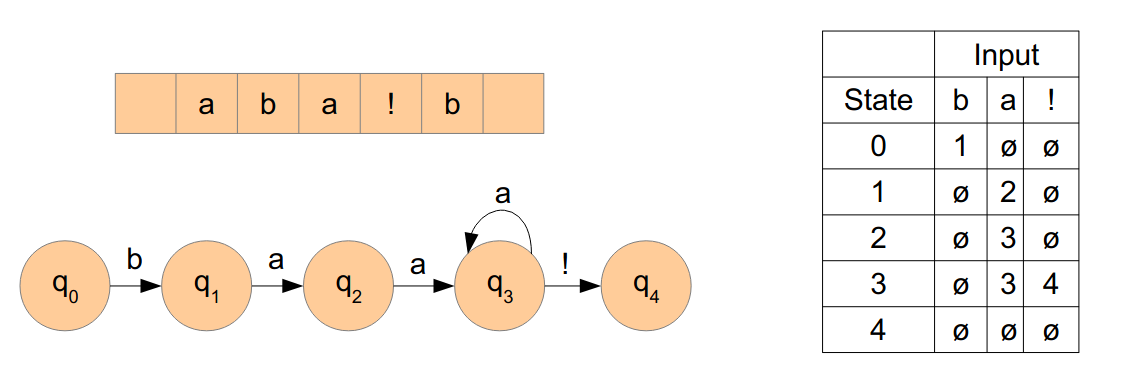
\includegraphics[width=\linewidth]{./images/fsa1.png}
			\label{fig:fsa1}
			\end{center}
	\end{figure}
	
	\begin{center}
	Figure \ref{fig:fsa1}: Example FSA representation
	\end{center}
	

	\item A deterministic FSA is one whose behaviour is fully determined by the state it is in and the input
	

	\item A non-deterministic FSA has an element of stochasticity; perhaps two paths for the same input, or an $\epsilon$ (i.e. spontaneous) transition 
	
	\item NDFSA's present challenges when determining whether a string should be accepted (by the language) as 'the wrong path' may be taken. A solution to this is to use a backtrack algorithm.
	
	\item Any NDFSA can be converted to a DFSA (See: parallel algorithm)
	
	\item An example of a DFSA suitable application is compiler scanning, and NDFSA is python RegEx
	
	

\end{itemize}
\newpage

\subsection{Regular Expressions}


Regular expressions are a powerful tool for pattern matching. 
They are one way to define an FSA, and also to define a formal (specifically regular) language. Any regular expression can be defined as an NDFSA and hence a DFSA \\


(Note: A formal language is a set of strings that are composed entirely from a finite symbol set $\Sigma$)

\subsection{Finite State Transducers}

\begin{itemize}
	\item A FST is a more general function than an FSA. It has two memory tapes, as opposed to FSA's one. 
	
	\item It 'reads' one string and generates another.
	
	\item Each 'state' can hold any value from the alphabet, and each outward arc contains a 'state/input' pair
	
	\begin{figure}[h!]
		\begin{center}
			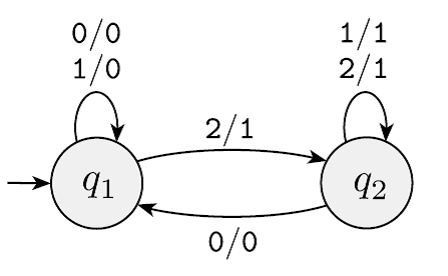
\includegraphics[width=0.5\linewidth]{./images/fst1.png}
			\label{fig:fst1}
		\end{center}
	\end{figure}
	
	\begin{center}
		Figure \ref{fig:fst1}: Example FST representation
	\end{center}
\end{itemize}







%\begin{figure}[h!]
%	\begin{center}
%		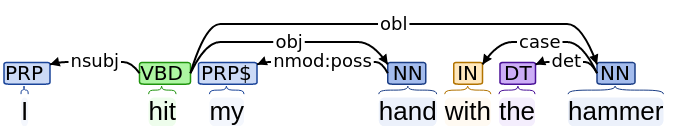
\includegraphics[width=0.6\linewidth]{./images/dependency.png}
%		\label{fig:dep1}
%		\end{center}
%\end{figure}

%\begin{center}
%Figure \ref{fig:dep1}: A typical dependency parse in (CoreNLP parse)
%\end{center}



\end{document}
